\subsection{Fliesskommazahlen}

\subsection{Addition}

\paragraph{Aufgabe \ref{ein_achtel}} Die maximale Zahl, die wir erreichen können, wenn wir \(1/8 + 1/8 + \dotsb + 1/8\) zusammen rechnen, ist \(4.0\).

Zum einen, wenn wir die \(4.0\) erreicht haben, kommen wir nicht mehr weiter.
Das sehen wir, wenn wir \(4.0 + 1/8\) ausrechnen. Wie gewöhnlich schreiben wir zuerst die Summanden untereinander.
\begin{figure}[H]
\centering
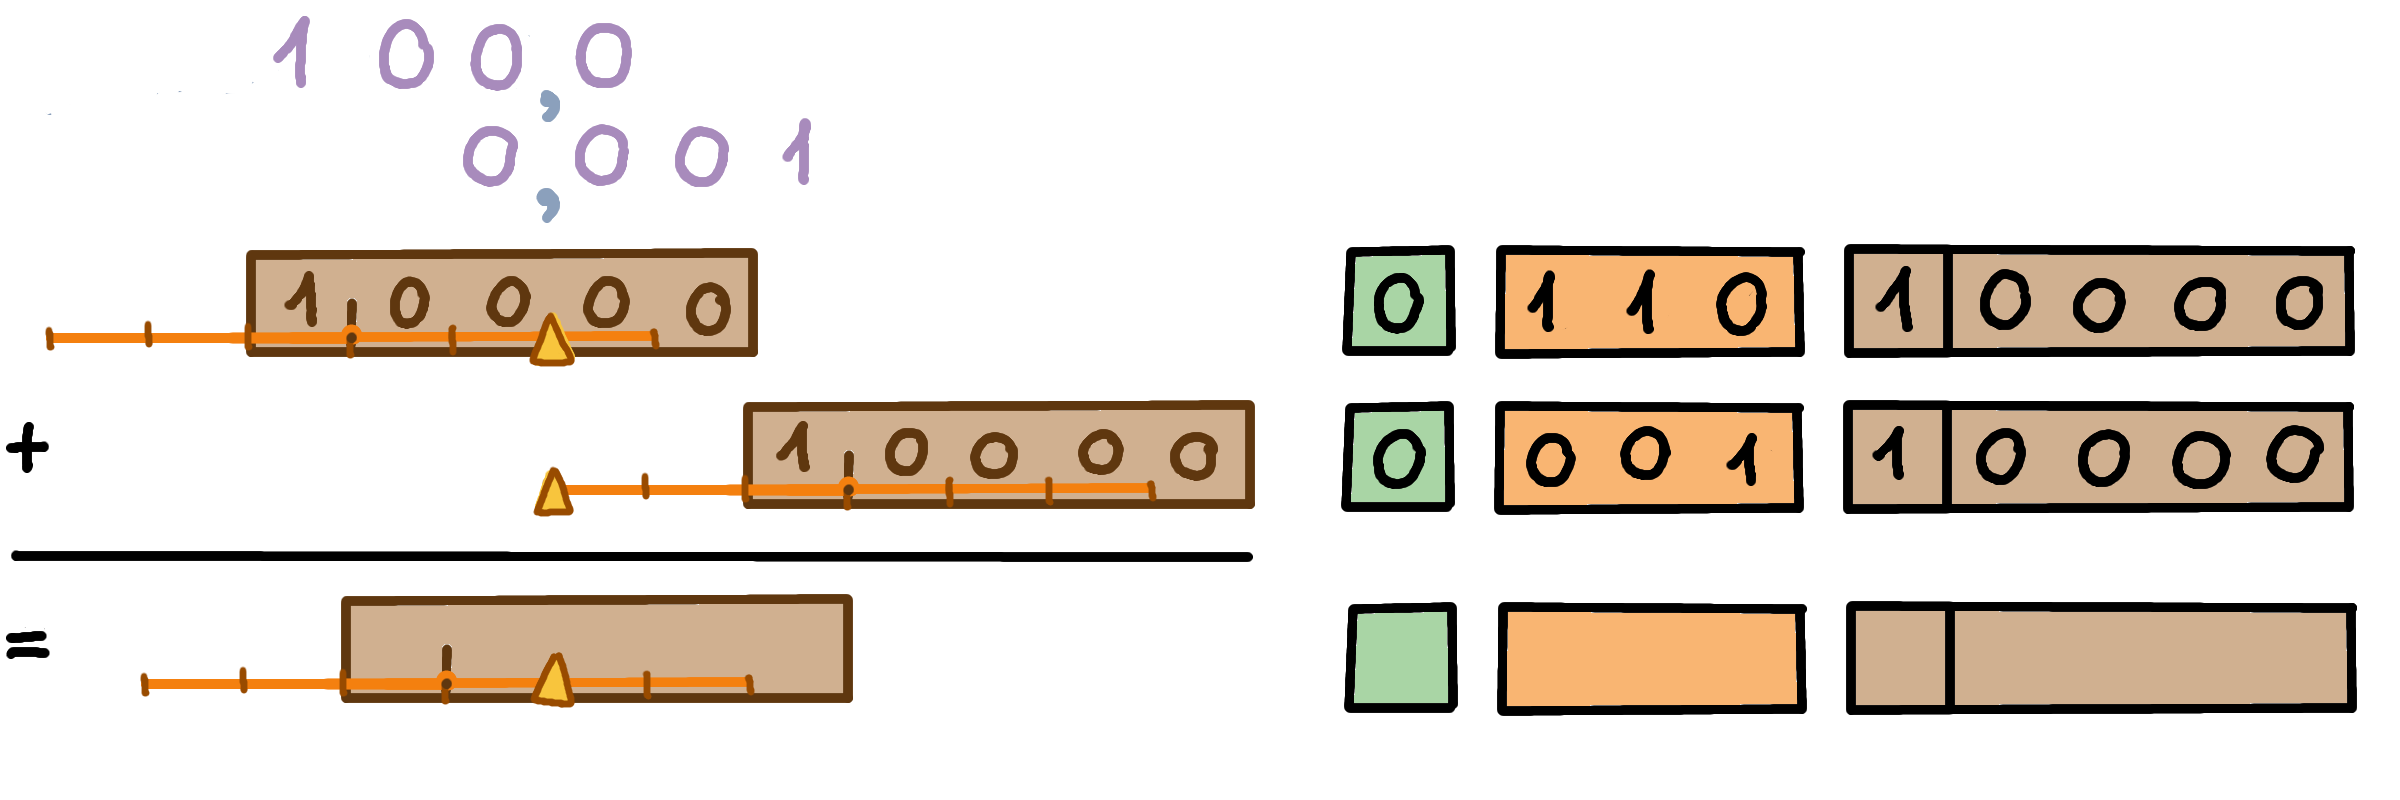
\includegraphics[width=\linewidth]{Pictures/Addition4and1-8_1.png}
\end{figure}
Wenn wir den Kasten von \(1/8\) unter den Kasten von \(4.0\) verschieben, sehen wir, dass alle signifikanten Stellen von \(1/8\) verloren gehen, auch die führende Eins.
\begin{figure}[H]
\centering
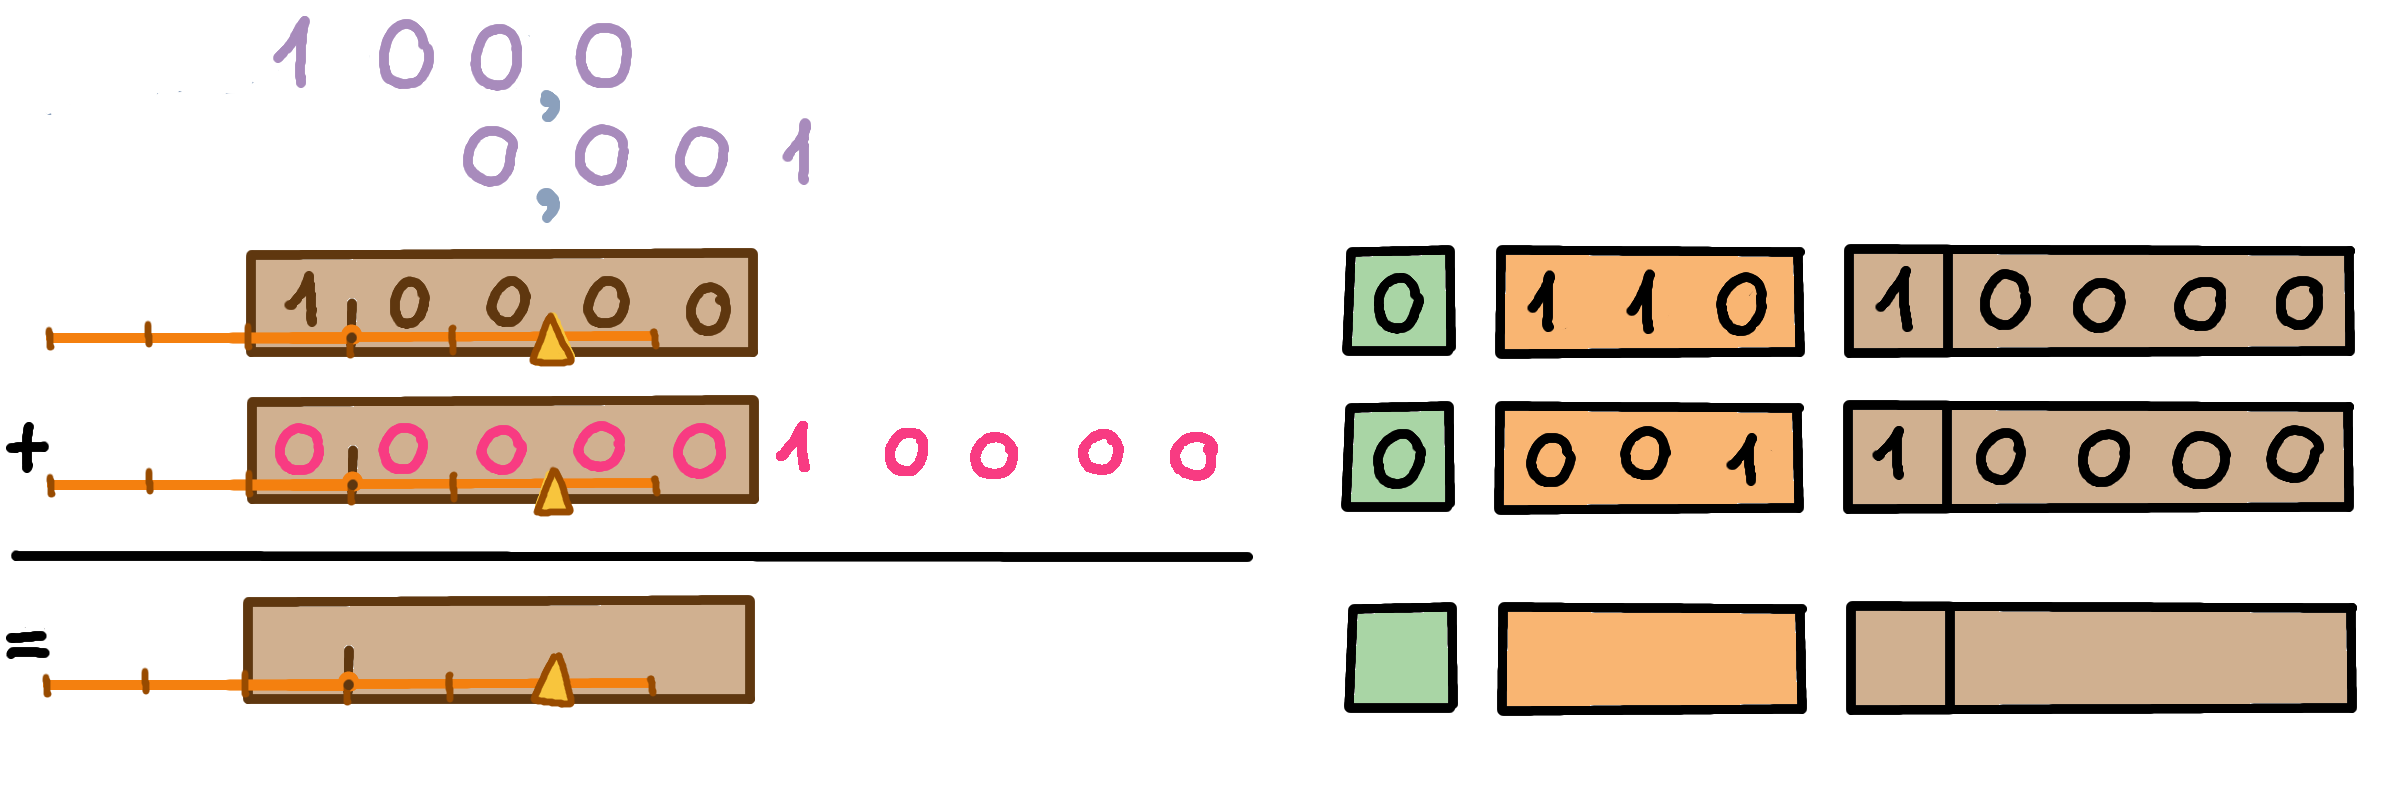
\includegraphics[width=\linewidth]{Pictures/Addition4and1-8_2.png}
\end{figure}
Deswegen, wenn wir \(4.0 + 1/8\) ausrechnen, kriegen wir \(4.0\).
\begin{figure}[H] 
\centering
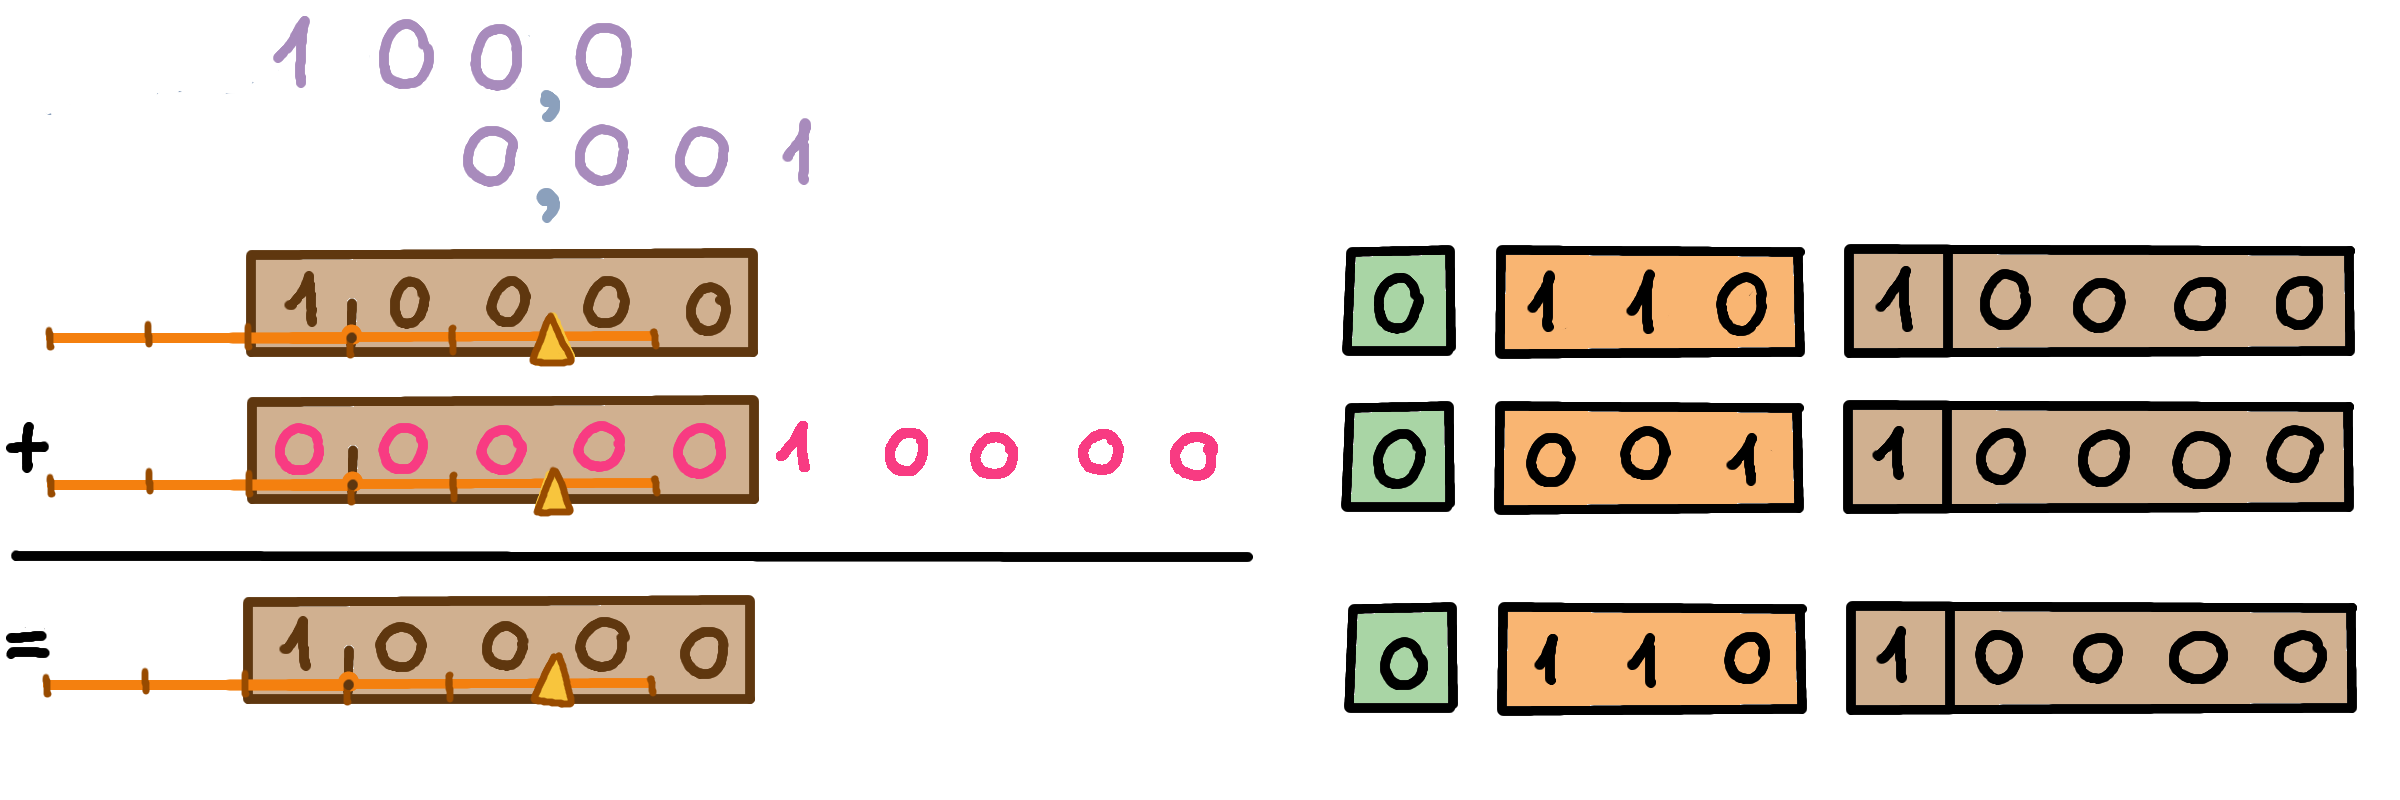
\includegraphics[width=\linewidth]{Pictures/Addition4and1-8_3.png} 
\end{figure}
Egal wie viele \(1/8\) rechnen wir zusammen, bleiben wir immer bei \(4.0\).

Jetzt bleibt uns zu zeigen, dass wir die \(4.0\) auch tatsächlich erreichen können. Das Problem bei der \(4.0\) ist, dass alle signifikanten Stellen von \(1/8\) verloren gehen. Das passiert, weil der Unterschied zwischen dem Exponenten von \(4.0\) und dem Exponenten von \(1/8\) die ganze Mantissenlänge beträgt. Das passiert bei einem kleineren Exponenten nicht. Zum Beispiel, wenn wir \(2.0 + 1/8\) ausrechnen, sehen wir, dass das Ergebnis wie erwartet \(17/8\) ist.

Um zu zeigen, dass das Problem erst bei \(4.0 + 1/8\) auftritt, rechnen wir \(2.0 + 1/8\). Das Ergebnis ist wie erwartet \(17/8\).
\begin{figure}[H]
\centering
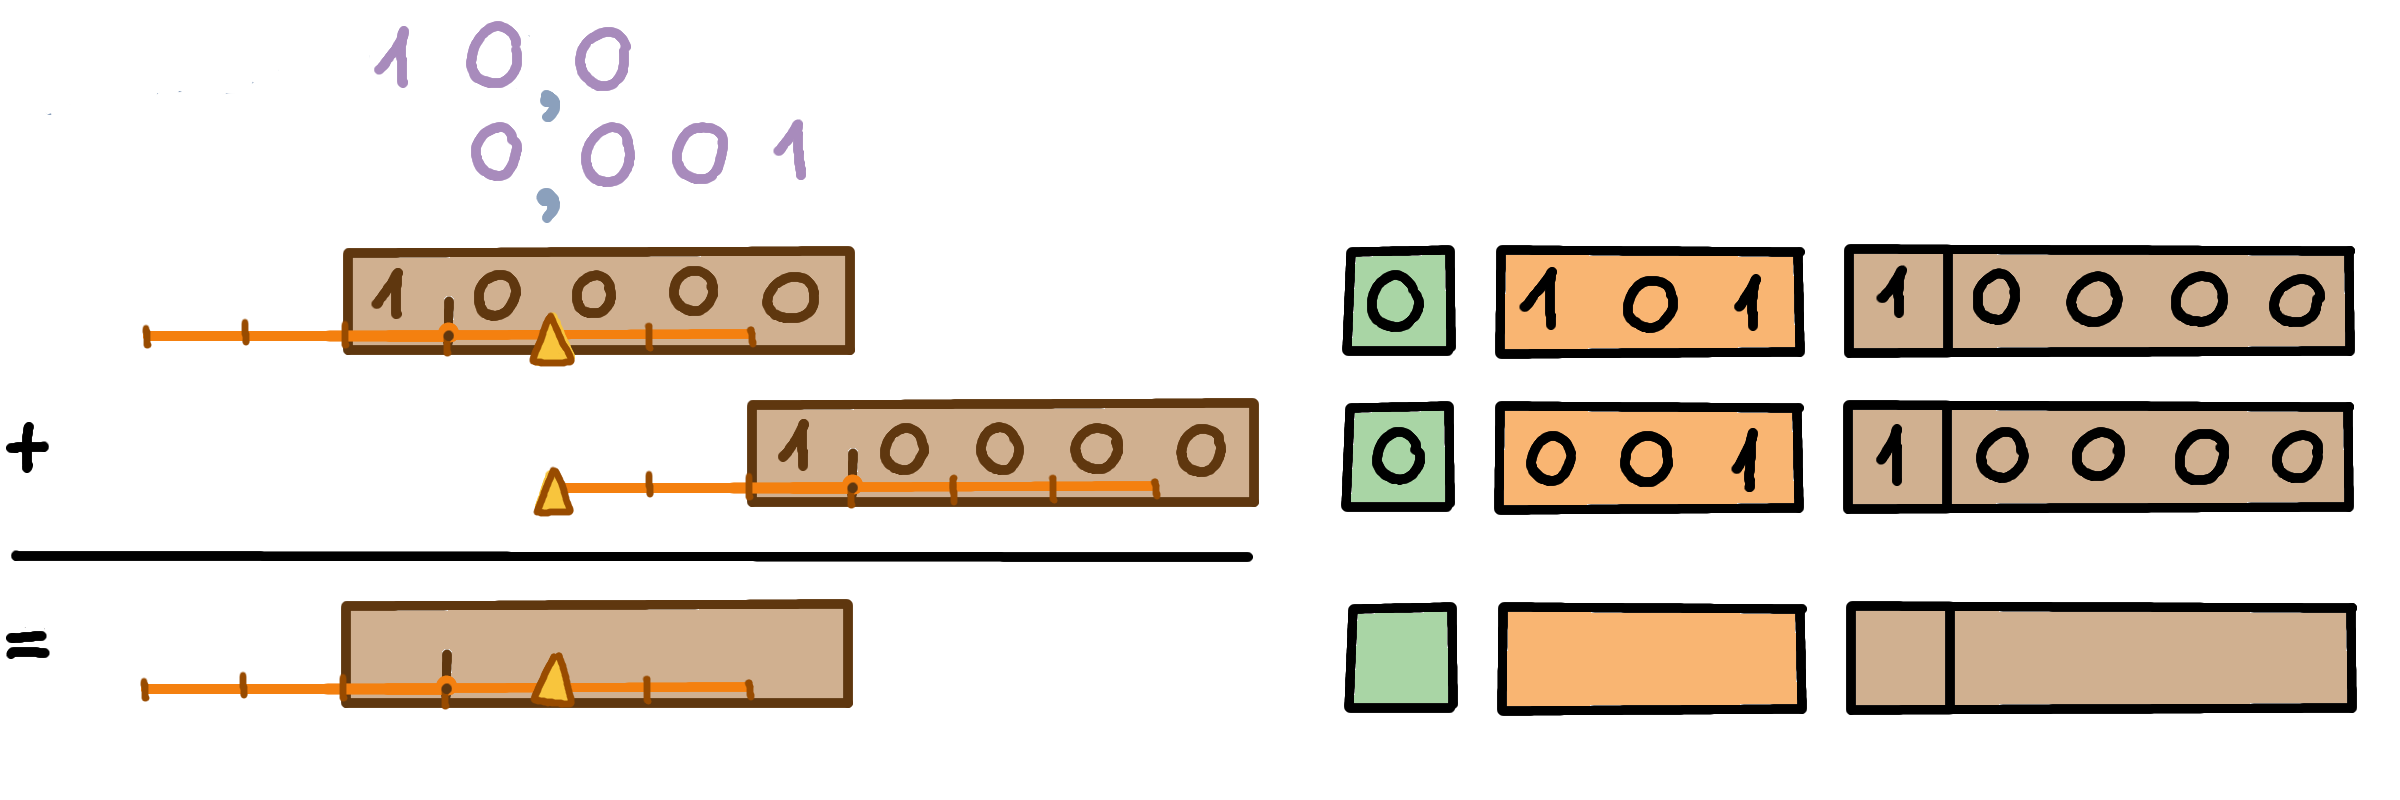
\includegraphics[width=\linewidth]{Pictures/Addition2and1-8_1.png} 
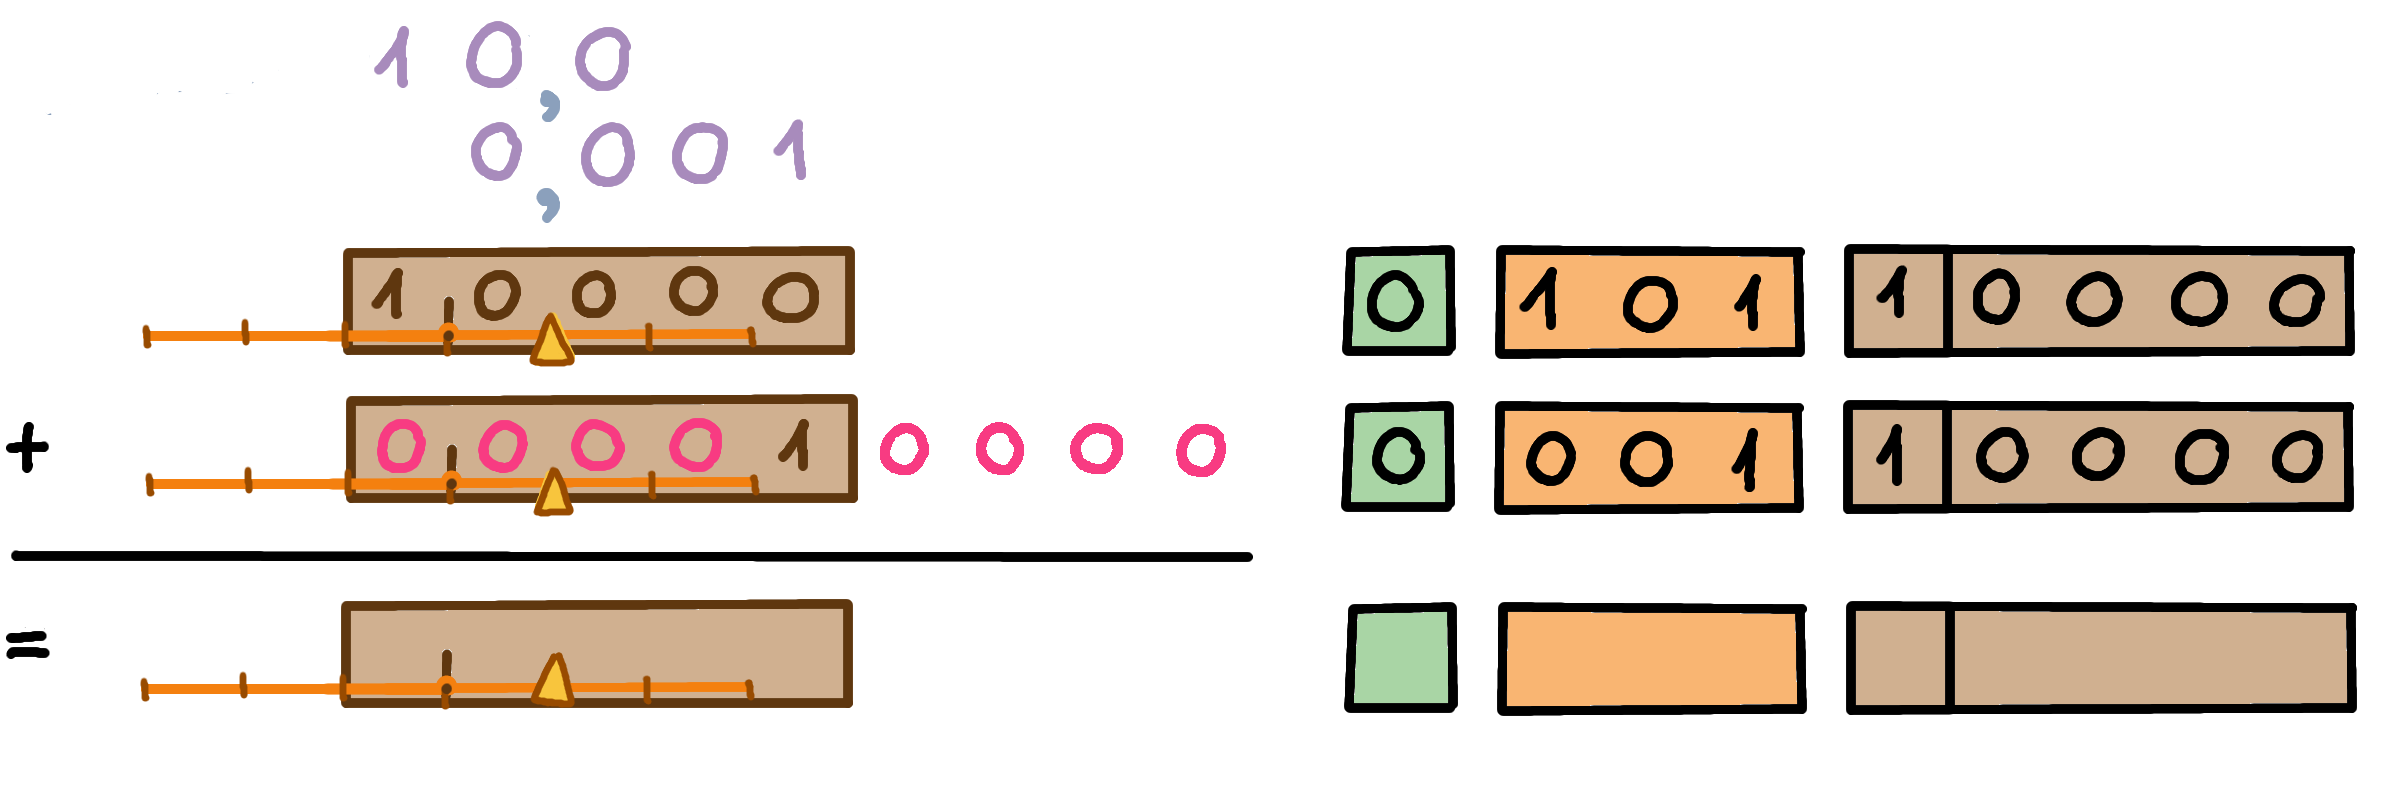
\includegraphics[width=\linewidth]{Pictures/Addition2and1-8_2.png} 
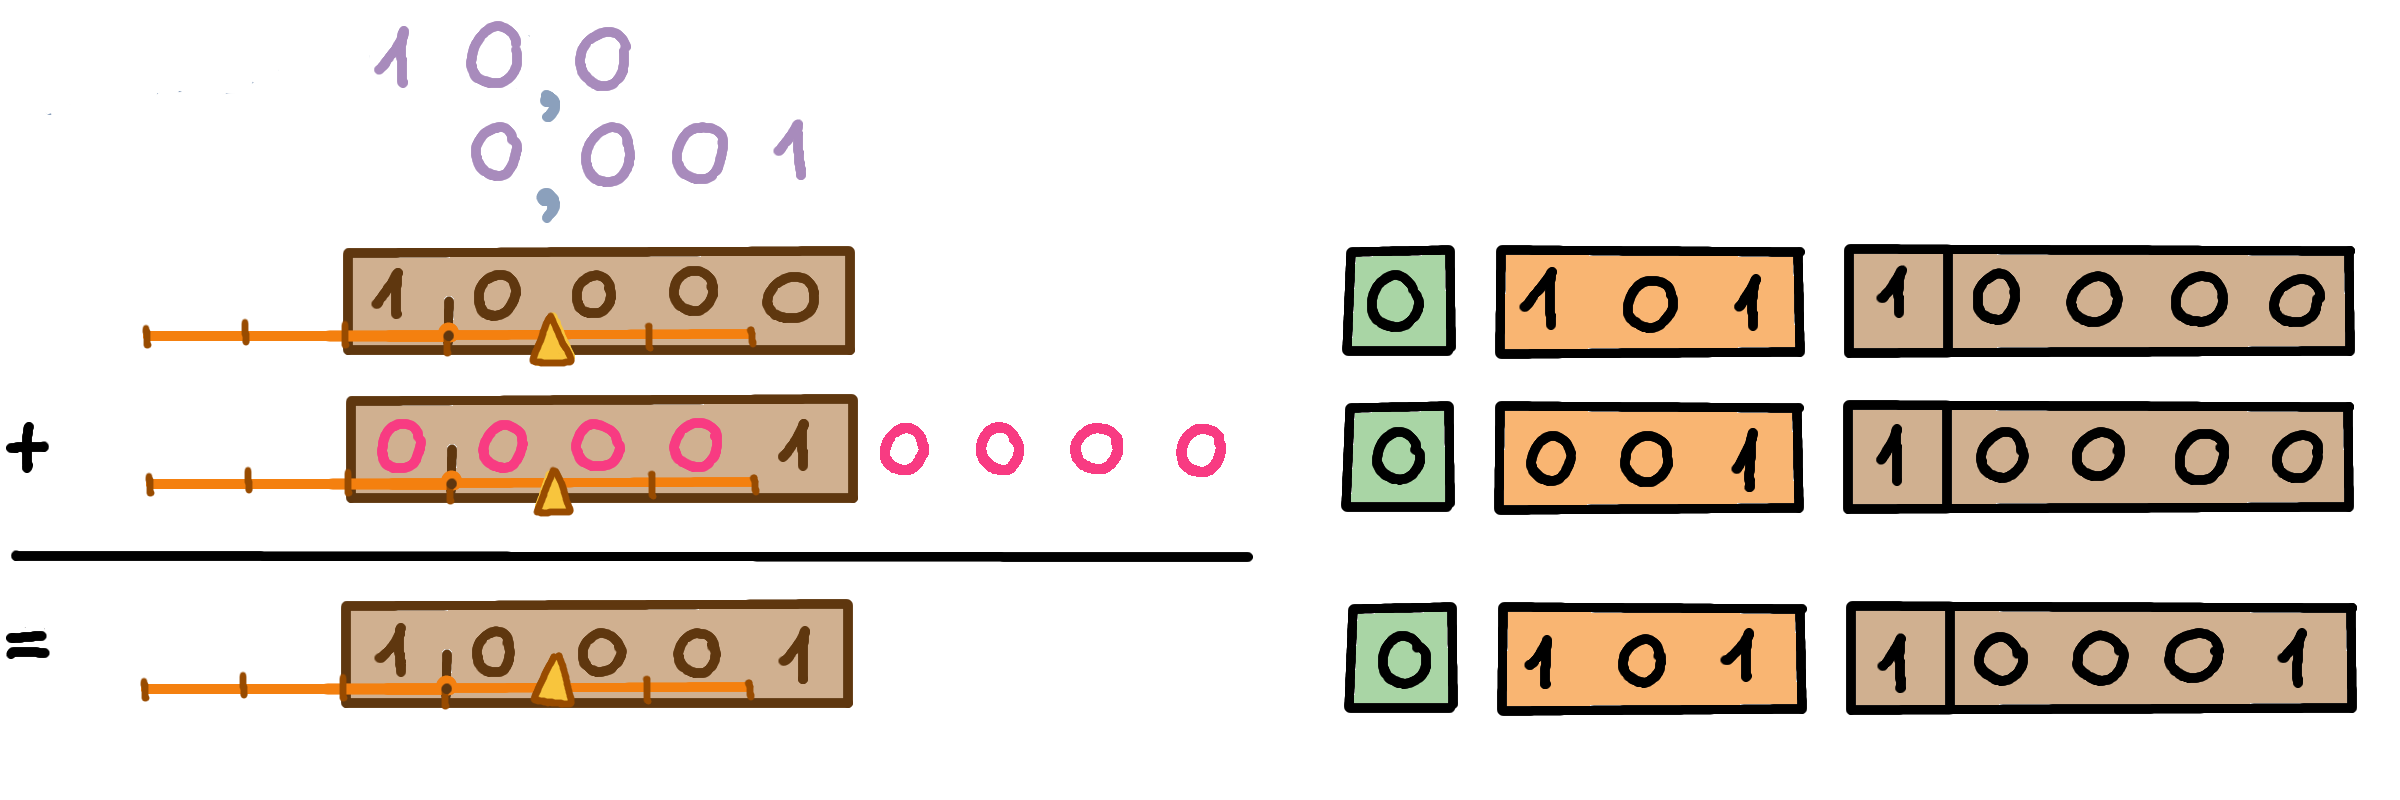
\includegraphics[width=\linewidth]{Pictures/Addition2and1-8_3.png} 
\end{figure}
Wir erreichen also die \(4.0\) nach 32 Summanden und kommen dann nicht mehr weiter.

%--------------------------------

\paragraph{Aufgabe \ref{addition_kontrollfragen}}


%--------------------------------

\paragraph{Aufgabe \ref{ameisenkönigin}}

Nein, das Programm der Ameisenkönigin wird unendlich lange laufen und die Anzahl Ameisen, die es braucht, um 10 Reiskörnchen zu transportieren, nie ausgeben. Das Problem ist analog zu dem, was wir in Aufgabe \ref{ein_achtel} gesehen haben. Das Programm läuft wie erwartet bis wir die \(8.0\) erreichen. Wenn wir aber \(1/4\) dazu rechnen, dann verlieren wir alle signifikanten Stellen von \(1/4\) und die \(8.0\) bleibt unverändert.
\begin{figure}[H]
\centering
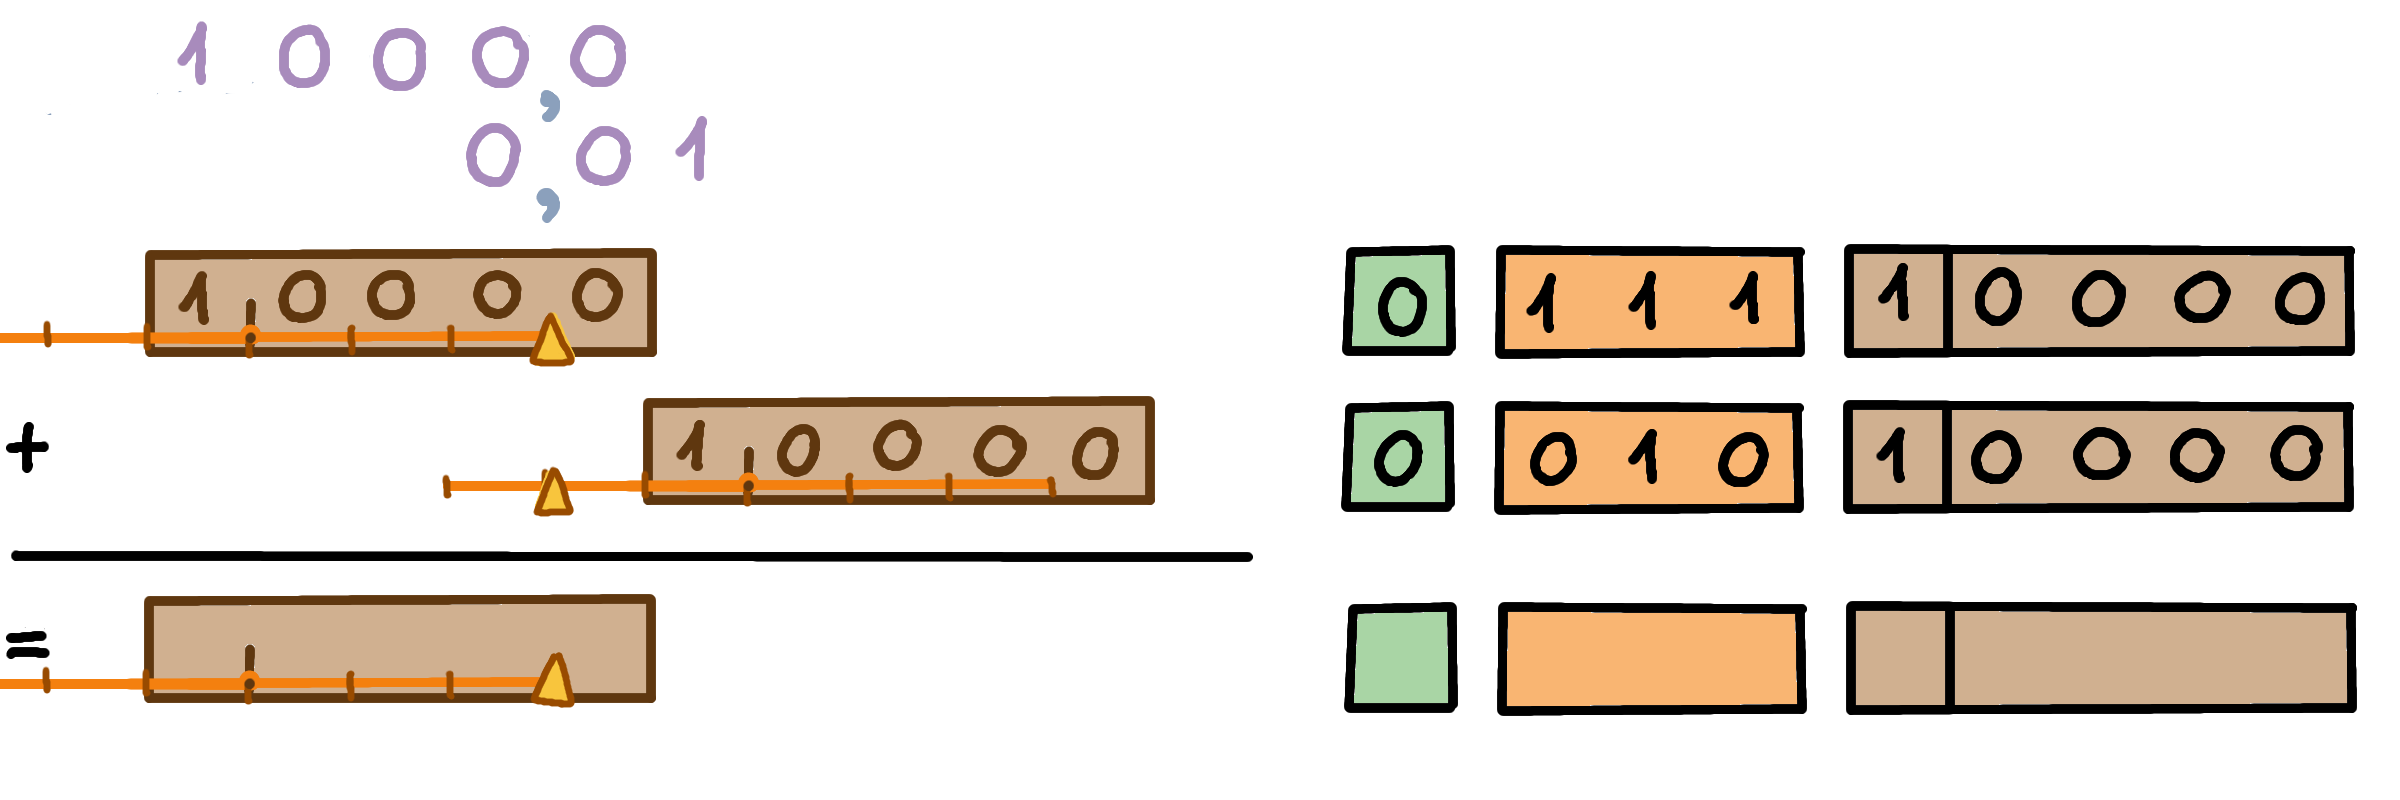
\includegraphics[width=\linewidth]{Pictures/Addition8and1-4_1.png} 
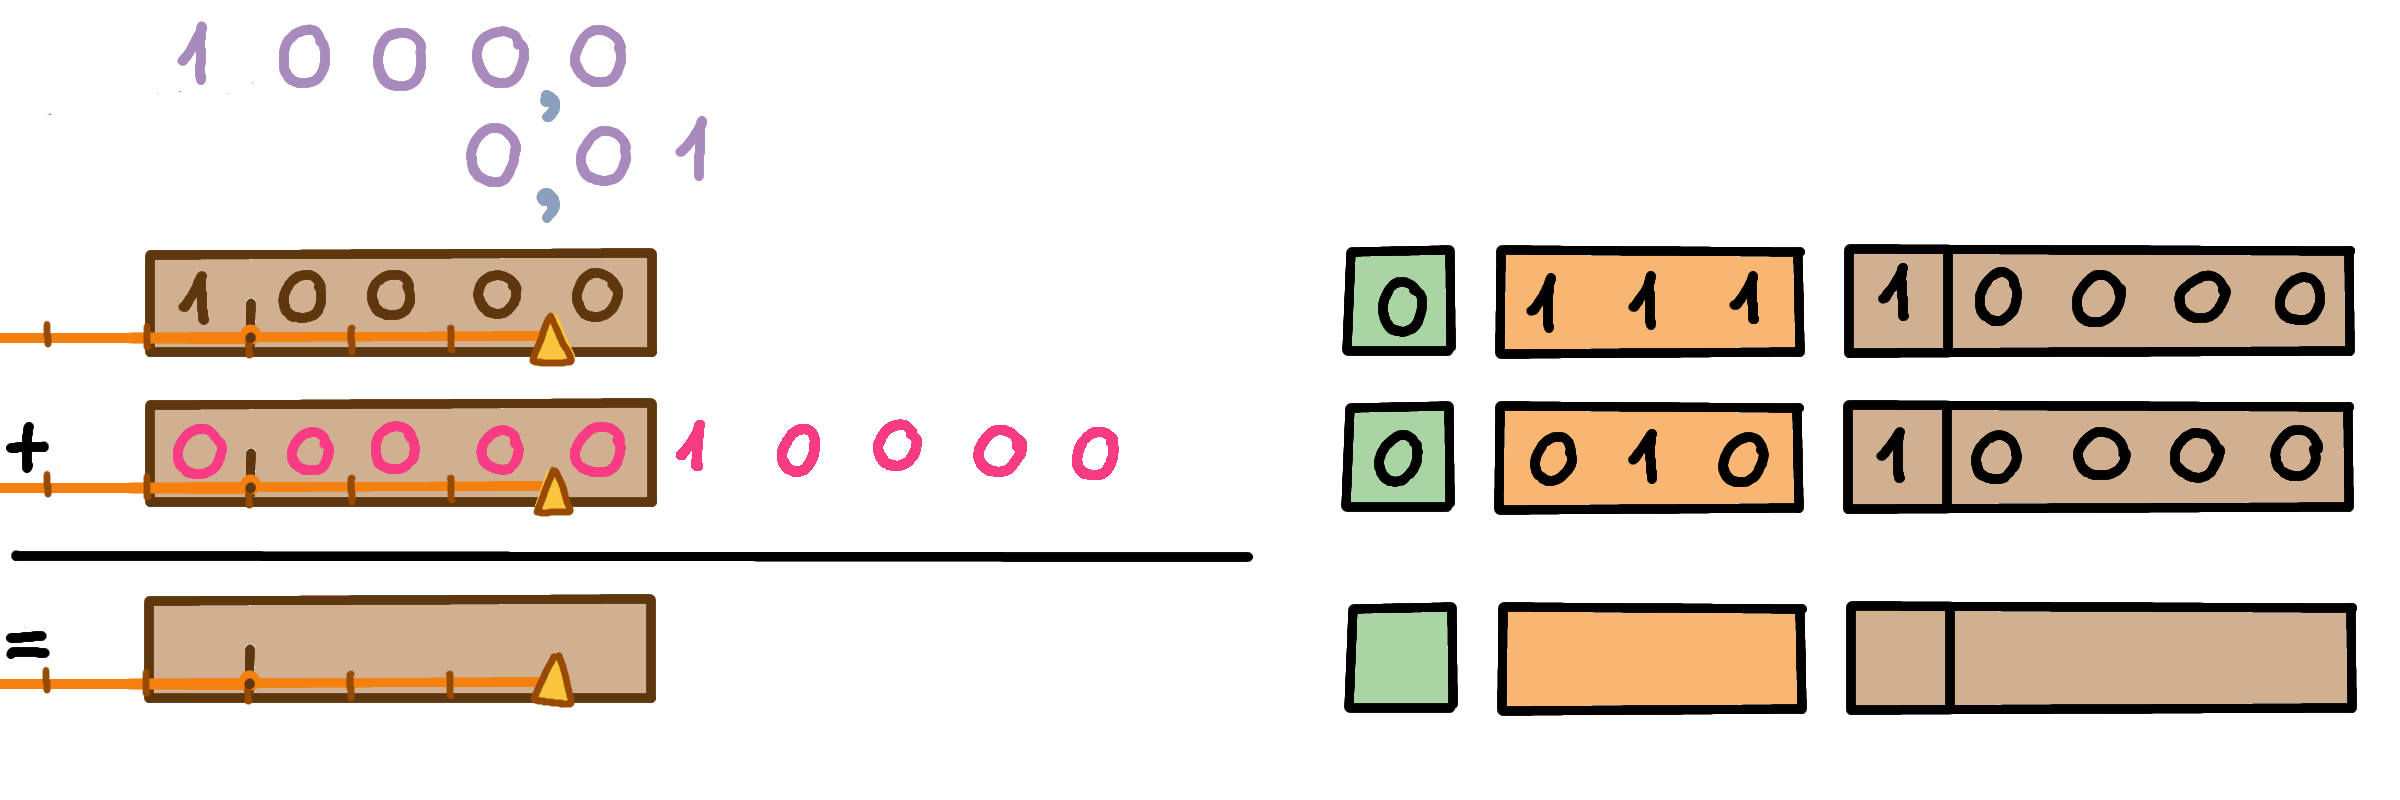
\includegraphics[width=\linewidth]{Pictures/Addition8and1-4_2.png} 
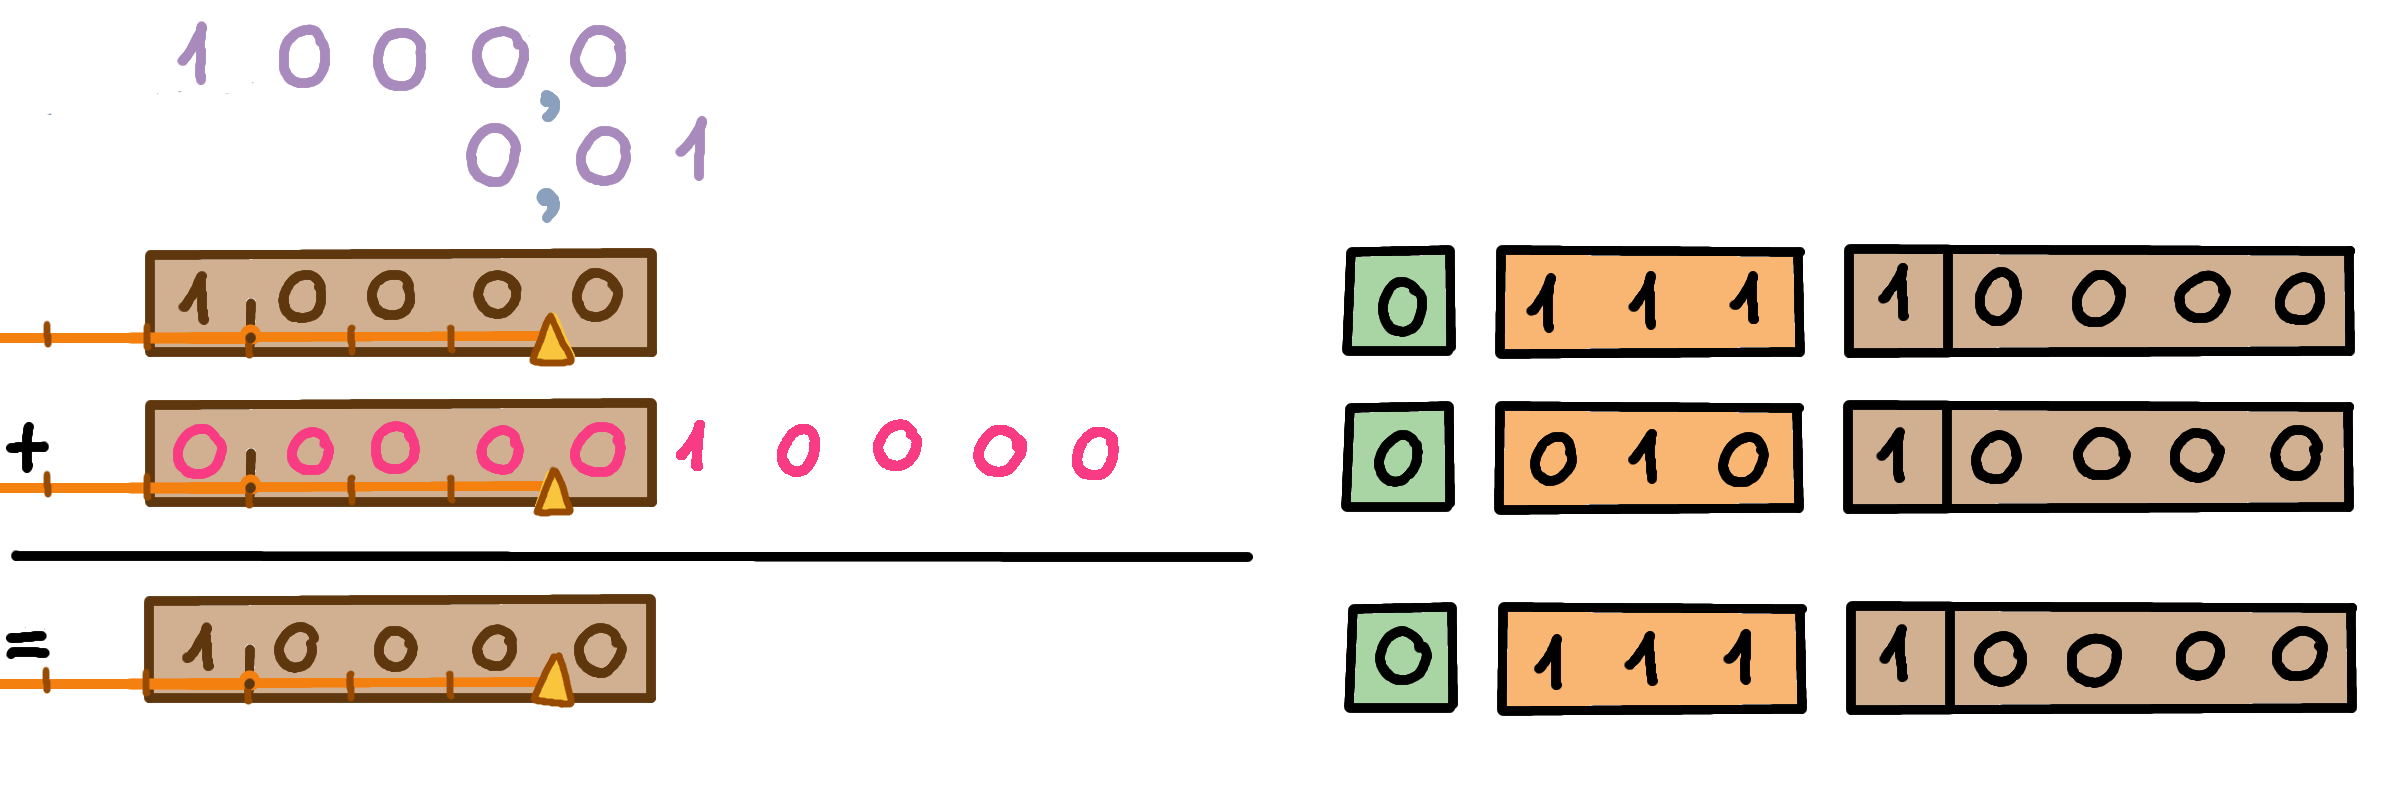
\includegraphics[width=\linewidth]{Pictures/Addition8and1-4_3.png} 
\end{figure}